\cotefile{150}
\scanpage{85}

\noindent\uline{16}\quad $\Sigma_J$ and $\Sigma_{J,L}$.

\margin{A perhaps more convenient point of view for defining the $\Sigma_i$, $\Sigma_{i_0-i_n}$, $\Sigma_J$, $\Sigma_J^{L}$ is that of ``oriented blow-ups'', better suited to formulas of the type $X=\underset{d\in\mathrm{Drap}(I)}{\uline{\lim}}\Sigma_d$ and so on. We take $\Sigma_i\supset X_i^*$ and not $\deleted{\unsure{\Sigma_i}}\subset X_i^*$, \unsure{likewise for} $\Sigma_J$, $X_J^*=\Sigma_J\setminus\dot\Sigma_J$\ldots}

Let $J$ be a band of $I$, we define
\[
(70)\qquad
\begin{array}{@{}l@{}}
\Sigma_J\subset X_J^*\\[-.4ex]
\hspace{.6em}\Vert\\[-.4ex]
X_J^*\unsure{\setminus|>}X_J^*\cap\displaystyle\bigcup_{i\in\bar J\setminus J}\mathring T_i
\end{array}
\]
\[
\begin{array}{@{}c@{\quad}l@{}}
\deleted{\Vert}&\Vert\quad\text{\uline{NB}}\\[-.4ex]
\deleted{\displaystyle\bigcup_{j\in J}\Sigma_j}&
X_J^{\deleted{\unsure{*}}}\setminus X_J^{\deleted{\unsure{*}}}\cap\displaystyle\bigcup_{i\in\bar J\setminus J}T_i
\end{array}
\]
\margin{NB $\bar J=$ ideal generated by $J$ $=\{i\in I\mid\exists j\in J\ \text{with}\ i\leq j\}$}
\margin{\uline{NB} We have set $X_J=\bigcup_{j\in J}X_j\ (=\bigcup_{j\in\bar J}X_j^*\unsure{=|\stackrel{?}{=}}X_J^*)$}

We therefore have
\[
(71)\quad\left\{
\begin{aligned}
\Sigma_{\phi}&=\phi,\quad\Sigma_{\{j\}}=\Sigma_j,\quad\Sigma_I=X\\
\Sigma_J&=X_J\quad\text{if $J$ an ideal i.e. $J=\bar J$}
\end{aligned}\right.
\]

We find, barring error
\[
(72)\qquad\Sigma_J\simeq\underset{i,j\in J}{\lim_{\longrightarrow}}\left(\Sigma_j,\Sigma_{ij},\deleted{\unsure{b}}(s_j,b_{ij}:\right.
\]
\diagram{\begin{tikzcd}[ampersand replacement=\&,column sep=small,row sep=small]
\&\Sigma_i\\
\Sigma_{ij}\arrow[ur,no head,to path={(\tikztostart.east)--([xshift=-3pt]\tikztotarget.west).. controls ([xshift=-1pt,yshift=1pt]\tikztotarget.west) and ([xshift=-1pt,yshift=-1pt]\tikztotarget.west)..([xshift=-3pt,yshift=-1pt]\tikztotarget.west)\tikztonodes}]\arrow[dr,no head,to path={(\tikztostart.east)--([xshift=-3pt]\tikztotarget.west).. controls ([xshift=-1pt,yshift=-1pt]\tikztotarget.west) and ([xshift=-1pt,yshift=1pt]\tikztotarget.west)..([xshift=-3pt,yshift=1pt]\tikztotarget.west)\tikztonodes}]\&\\
\&\Sigma_j
\end{tikzcd}}
\[
\left.\vphantom{\Sigma_{ij}}\right)\qquad\simeq\underset{d\in\mathrm{Drap}(J)}{\uline{\lim}}\Sigma_d
\]
\margin{\uline{NB} $\Sigma_J$ is endowed with a stratification of type $J$, which \unsure{one deduces} \unsure{to the|from the} $(\Sigma_j,\Sigma_{jh},s_{jh},b_{jh})$ \unsure{with|where} $\unsure{\forall|j,}h\in I$}
\deleted{As a result \unsure{of a}}
\[
(73)\qquad\Sigma_J\overset{\overset{h}{\sim}}{\hookrightarrow}X_J^*\qquad\substack{\text{(homo-}\\\text{topy equivalence)}}
\]

We set
\[
(74)\qquad\begin{aligned}
\dot\Sigma_J&=X_J\cap\left(\text{boundary of }\underset{\displaystyle\bigcup_{i\in\bar J-J}T_i}{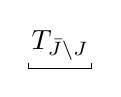
\begin{tikzpicture}[baseline=(term.base)]
\node[inner sep=1pt] (term) {$T_{\bar J\setminus J}$};
\draw ([yshift=.5pt]term.south west)--([yshift=-1.5pt]term.south west)--([yshift=-1.5pt]term.south east)--([yshift=.5pt]term.south east);
\end{tikzpicture}}\right)\\
&=\bigcup_{\substack{i<j\\i,j\in J}}\operatorname{Im}(\Sigma_{ij}\to\Sigma_J)\\
&=\underset{\substack{d\in\mathrm{Drap},\ d\text{ \unsure{with|having} at least 2 terms}}}{\lim_{\twoheadrightarrow}}\Sigma_d
\end{aligned}
\]
% Thin lower foliation, in another hand; not the author's page number.
\margin{84}
